% Final report: pattern-agnostic multispectral demosaicking.
% Based on the ICIP-2026 template; to be used with:
%          spconf.sty  - ICASSP/ICIP LaTeX style file, and
%          IEEEbib.bst - IEEE bibliography style file.
% Every number in this report comes from ../results/ (summary.csv,
% per_scene.csv, hypotheses.json), from ../results_arad/ (cross-dataset
% protocol, Section 5.4) or from docs/revision-2026-11-16.md.
% Compile from this folder:  tectonic report.tex
% --------------------------------------------------------------------------
\documentclass{article}
\usepackage[hyphens]{url}
\usepackage{spconf,amsmath,amssymb,graphicx,tikz,array,multirow}
\newcolumntype{L}[1]{>{\raggedright\arraybackslash}p{#1}}
\newcolumntype{C}[1]{>{\centering\arraybackslash}p{#1}}
\usetikzlibrary{arrows.meta,positioning,fit}
\graphicspath{{../results/figs/}}

% Notation.
% ---------
\def\X{{\mathbf X}}
\def\Y{{\mathbf Y}}
\def\C{{\mathbf C}}
\def\M{{\mathbf M}}
\def\N{{\mathbf N}}
\def\x{{\mathbf x}}
\newcommand{\wb}{\mathrm{WB}}
\newcommand{\seen}[1]{\underline{#1}}

% Spectral palette used to draw the MSFA patterns (band 1 = violet, 16 = red).
\definecolor{b1}{HTML}{5B3FD0}\definecolor{b2}{HTML}{4F4FD8}
\definecolor{b3}{HTML}{3F62DC}\definecolor{b4}{HTML}{2A75DB}
\definecolor{b5}{HTML}{1E88D0}\definecolor{b6}{HTML}{1A99B8}
\definecolor{b7}{HTML}{1BA49B}\definecolor{b8}{HTML}{2DAE7A}
\definecolor{b9}{HTML}{5BB55A}\definecolor{b10}{HTML}{8FBC40}
\definecolor{b11}{HTML}{C2C036}\definecolor{b12}{HTML}{E3B935}
\definecolor{b13}{HTML}{E8A030}\definecolor{b14}{HTML}{E8822C}
\definecolor{b15}{HTML}{DD5E31}\definecolor{b16}{HTML}{C93A3A}

% \msfa{expr}: draws a 16x16 crop of an MSFA; expr gives the band (1..16)
% of the pixel in row \i and column \j (both 0-based).
\newcommand{\msfa}[1]{%
  \begin{tikzpicture}[x=0.118cm,y=0.118cm]
    \foreach \i in {0,...,15}{
      \foreach \j in {0,...,15}{
        \pgfmathtruncatemacro{\b}{#1}
        \edef\c{b\b}
        \fill[fill=\c] (\j,-\i) rectangle ++(1,-1);
      }
    }
    \draw[black!60, line width=0.3pt] (0,0) rectangle (16,-16);
  \end{tikzpicture}}

% Title.
% ------
\title{ONE NETWORK FOR ANY FILTER ARRAY:\\
  PATTERN-AGNOSTIC MULTISPECTRAL DEMOSAICKING}
%
\name{Benjam\'in Cisternas, Gonzalo Michea}
\address{Computational Photography 2026-2\\
  Departamento de Inform\'atica, Universidad T\'ecnica Federico Santa Mar\'ia\\
  Valpara\'iso, Chile}
%
\begin{document}
%
\maketitle
%
\begin{abstract}
Snapshot multispectral cameras use a multispectral filter array (MSFA), so
each pixel measures one of 16 bands and about 94\% of the datacube must be
estimated. Learned demosaicking networks give the best results but must be
retrained for each MSFA. We condition a small U-Net on the pattern, by
feeding it a bilinear estimate, the sparse measurements and the mask, and
train it on random balanced patterns. We test it with four MSFAs never used
to train it (IMEC, optimal sphere packing, BTES and a random kernel). On
held-out CAVE scenes, networks trained for one pattern lose 7.4 to 15.5\,dB
on the other patterns and fall below bilinear interpolation. The single
agnostic network stays within 1.2 to 1.4\,dB of each specialized network on
its own pattern and is 6.3 to 9.9\,dB better on unseen patterns. Training on
ARAD-1K and testing on all 32 CAVE scenes confirms these findings, but also
shows a dataset gap that affects every learned method.
\end{abstract}
%
\begin{keywords}
Multispectral imaging, multispectral filter array, demosaicking, deep
learning, generalization
\end{keywords}
%
% ==========================================================================
\section{Introduction}
\label{sec:intro}
% ==========================================================================

A color camera records three values per pixel, but the reflectance spectra
of most materials contain much more information than three numbers.
Multispectral imaging (MSI) samples the spectrum in several narrow bands,
typically 8 to 32 in the visible and near-infrared range. The result is a
\emph{datacube} with two spatial dimensions and one spectral dimension. The
spectrum of each pixel helps to distinguish materials that look alike in RGB,
so MSI is used in remote sensing~\cite{diaz2023}, medical
imaging~\cite{lu2014}, agriculture, food inspection and cultural heritage.

The difficulty of MSI is acquisition: a 2D sensor cannot record a 3D datacube
in one exposure without a trade-off. Scanning cameras record the cube one line
or one band at a time, which is slow and fails with moving scenes. Snapshot
cameras based on a \emph{multispectral filter array} (MSFA) trade spatial
sampling for speed: a mosaic of narrow-band filters covers the sensor and each
pixel measures a single band~\cite{lapray2014,geelen2014}. A
\emph{demosaicking} algorithm must then estimate the missing values. With
$L=16$ bands, each band is measured at only $1/16$ of the pixels, so about
94\% of the datacube is unknown. This is far harder than RGB demosaicking,
where green is measured at half of the pixels. Demosaicking is therefore a
central computational photography problem: the camera is only useful together
with the algorithm that reconstructs its images.

Two lines of research have improved MSFA cameras. The first designs better
patterns: Diaz et al.~\cite{diaz2023} recently placed the filters by
\emph{optimal sphere packing} (OSP) in the spatio-spectral domain and reported
up to 2\,dB of improvement over seven existing MSFAs. The second learns the
reconstruction with convolutional neural networks, which clearly outperform
classical interpolation~\cite{feng2021,diaz2023}. These two lines do not fit
well together. A network receives only the raw mosaic, learns the pattern
implicitly, and becomes tied to the MSFA used in training. In~\cite{diaz2023}
the network was retrained for every pattern, about a day and a half on two
GPUs each time, and the authors state that ``a significant limitation of the
proposed method is the necessity of retraining for specific MSFAs''. This
dependence is costly: comparing $n$ candidate patterns requires $n$ trained
networks, and a camera with a new or slightly different pattern needs a new
model.

\textbf{Research question.} \emph{Can a single demosaicking network
reconstruct multispectral images from any MSFA, including patterns not seen
during training, with a quality close to that of a network trained for each
pattern?} We test three hypotheses:
\begin{itemize}
  \item[\textbf{H1}] A network trained for one pattern degrades strongly on
        unseen patterns.
  \item[\textbf{H2}] A pattern-agnostic network stays within 2\,dB of each
        pattern-specific network on that network's own pattern. Our written
        proposal used a stricter 1\,dB threshold; we report both.
  \item[\textbf{H3}] On unseen patterns, the agnostic network outperforms
        both the pattern-specific networks and bilinear interpolation.
\end{itemize}

\textbf{Contributions.} (i) An open Python pipeline for simulated MSFA
demosaicking, verified against the public code of~\cite{diaz2023}: our
patterns match theirs pixel by pixel, and our weighted bilinear baseline
reproduces their reported PSNR within 0.13\,dB. (ii) A systematic
measurement of how much learned demosaicking depends on the training
pattern. (iii) A pattern-agnostic network for 16-band MSFAs: a U-Net
conditioned on the pattern through its input and trained on random balanced
patterns, which extends random-pattern training, previously shown for RGB
filter arrays~\cite{bourrier2022}, to a setting with 94\% missing values
instead of two thirds. (iv) An ablation
of the network input, which shows that a pattern-aware interpolation as input
is the key ingredient. Without it, the agnostic network stays below bilinear
interpolation at the same training budget. (v) A cross-dataset experiment
(training on ARAD-1K, testing on all 32 CAVE scenes) that confirms the
results with four times more test scenes.

% ==========================================================================
\section{Background and related work}
\label{sec:background}
% ==========================================================================

\subsection{Image formation}

We denote the datacube by $\X\in\mathbb{R}^{H\times W\times L}$. Its $k$-th
band $\X_k\in\mathbb{R}^{H\times W}$ is the scene seen through a narrow
filter centered at wavelength $\lambda_k$, and $\x(m,n)\in\mathbb{R}^L$ is
the spectrum at pixel $(m,n)$. An MSFA assigns one band to every pixel. Let
$\C_k\in\{0,1\}^{H\times W}$ be the binary mask of band $k$, with
$\sum_k\C_k=\mathbf{1}$. With ideal narrow-band filters, the sensor records
the mosaic~\cite{diaz2023}
\begin{equation}
  \Y = \sum_{k=1}^{L} \X_k \odot \C_k + \N,
  \label{eq:model}
\end{equation}
where $\odot$ is the element-wise product and $\N$ is sensor noise. The
one-hot mask $\M=[\C_1,\dots,\C_L]\in\{0,1\}^{H\times W\times L}$ fully
describes the pattern, and $\Y\odot\M$ (with $\Y$ broadcast over bands) is the
\emph{sparse cube} that places each measurement in its own band.
Demosaicking estimates $\X$ from $\Y$. Eq.~\eqref{eq:model} gives $HW$
equations for $HWL$ unknowns, so the problem is severely ill-posed and every
method needs a prior on natural images. The usual priors are spatial
correlation (neighboring pixels are similar) and spectral correlation (bands
with close wavelengths are similar). When the prior fails, three artifacts
appear: \emph{zipper} patterns that follow the period of the filter kernel,
\emph{false colors} (spectra that do not exist in the scene) and
\emph{blur}~\cite{diaz2023}.

\subsection{MSFA design}

Like the Bayer array~\cite{bayer1976}, most MSFAs repeat a small kernel. For
example, commercial IMEC sensors tile a $4\times4$ kernel with 16
bands~\cite{geelen2014}. Other designs include random (RND) and sequential
kernels, the Brauers--Aach pattern~\cite{brauers2006} and the
binary-tree-based edge-sensing pattern (BTES)~\cite{miao2006}. Hirakawa and
Wolfe~\cite{hirakawa2008} gave one of the first principled criteria, in the
Fourier domain, for color filter arrays. Diaz et al.~\cite{diaz2023} represent
every sampled pixel as a point (row, column, band) in an $L\times L\times L$
cube and ask for points that are as far apart as possible, which is a sphere
packing problem. On a sensor grid they restrict the search to lattices
\begin{equation}
  B(i,j) = \big((a\,i + b\,j)\bmod L\big) + 1,
  \label{eq:osp}
\end{equation}
where $i,j$ are the 1-based row and column indices. The best pair for $L=16$
is $a=7$, $b=4$. This OSP pattern has a sphere diameter of 2.45 and a
packing density of 0.40, against 1.41 and 0.08 for IMEC and 1.73 and 0.14
for BTES~\cite{diaz2023}. Note that OSP repeats every 16 rows and every 4
columns, so unlike IMEC and BTES it is not a tiled $4\times4$ kernel.
Fig.~\ref{fig:patterns} shows the four patterns used in this work.

\begin{figure}[t]
\centering
\begin{minipage}[b]{0.24\linewidth}
  \centering
  \msfa{{7,8,6,5,15,16,14,13,11,12,10,9,3,4,2,1}[4*mod(\i,4)+mod(\j,4)]}
  \centerline{\small (a) IMEC}
\end{minipage}\hfill
\begin{minipage}[b]{0.24\linewidth}
  \centering
  \msfa{mod(7*(\i+1)+4*(\j+1),16)+1}
  \centerline{\small (b) OSP}
\end{minipage}\hfill
\begin{minipage}[b]{0.24\linewidth}
  \centering
  \msfa{{1,13,4,15,9,5,11,7,3,16,2,14,12,8,10,6}[4*mod(\i,4)+mod(\j,4)]}
  \centerline{\small (c) BTES}
\end{minipage}\hfill
\begin{minipage}[b]{0.24\linewidth}
  \centering
  \msfa{{11,3,14,6,1,9,16,4,13,7,2,12,5,15,8,10}[4*mod(\i,4)+mod(\j,4)]}
  \centerline{\small (d) Random}
\end{minipage}
\caption{$16\times16$ crops of the four test MSFAs with $L=16$ (color =
band, from violet at 400\,nm to red at 700\,nm). (a) IMEC $4\times4$
kernel~\cite{geelen2014}; (b) sphere-packing lattice of Eq.~\eqref{eq:osp}
with $a=7$, $b=4$~\cite{diaz2023}; (c) BTES~\cite{miao2006}; (d) a fixed
random $4\times4$ kernel. (a)--(c) match the public code of~\cite{diaz2023}
pixel by pixel.}
\label{fig:patterns}
\end{figure}

\subsection{Classical demosaicking}

\textbf{Weighted bilinear (WB)} interpolation~\cite{brauers2006}
interpolates each sparse band $\Y\odot\C_k$ independently with a normalized
low-pass kernel. It is fast and pattern independent, but it ignores spectral
correlation and blurs edges. \textbf{Spectral-difference} methods interpolate
the smoother difference between two bands instead of the bands
themselves~\cite{brauers2006,mizutani2014}. \textbf{Intensity-guided}
methods first estimate an image that combines all bands, such as the
pseudo-panchromatic image of PPID~\cite{mihoubi2017}, and interpolate each
band relative to it. Demosaicking can also be posed as a regularized inverse
problem, for example with low-rank and graph priors~\cite{tsagkatakis2019}.

\subsection{Learned demosaicking}

A network $f_\theta$ is trained on pairs $(\Y,\X)$ simulated with
Eq.~\eqref{eq:model} from datacubes captured by scanning cameras. Examples
are the mosaic convolution-attention network (MCAN)~\cite{feng2021} and
TRevSCI~\cite{diaz2023}, an adaptation of a reversible network for snapshot
compressive imaging~\cite{cheng2021}. For RGB, Gharbi et
al.~\cite{gharbi2016} showed that joint demosaicking and denoising with one
network works better than solving the two steps separately. The NTIRE 2022
spectral demosaicing challenge~\cite{arad2022demosaic} benchmarked learned
methods on 16-channel MSFA images. In~\cite{diaz2023}, TRevSCI improves on
WB by 5 to 8\,dB, but it receives only $\Y$ and was retrained for each
of the eight MSFAs studied.

\subsection{Pattern-independent demosaicking}

For RGB color filter arrays (CFAs), several methods work with any pattern.
Zhang et al.~\cite{zhang2016} proposed a classical universal demosaicking
method for periodic and aperiodic CFAs, and Stojkovi\'c et
al.~\cite{stojkovic2019} used CFA-agnostic algorithms to compare CFA
layouts. Henz et al.~\cite{henz2018} learn the CFA jointly with the network,
which is then tied to the learned pattern. Closest to our work, Bourrier et
al.~\cite{bourrier2022} trained a CNN on randomly mosaicked RGB images and
found that it performs equally well on periodic and on other random mosaics.
Bai et al.~\cite{bai2024} handle arbitrary sparse CFAs with a network whose
first operation is a scatter-weighted interpolation. For MSFAs, generic
methods are mostly classical: WB and PPID work with any pattern, and Bian et
al.~\cite{bian2021} proposed a generalized nonlocal low-rank method, noting
that existing methods suffer from limited accuracy or poor generalization.
Wang and Davies~\cite{wang2026} recently described a self-supervised
multispectral method that does not depend on a specific pattern, but they
evaluate it on a single $4\times4$ MSFA.

Two ideas from other problems are also relevant.
\emph{Normalized convolution}~\cite{knutsson1993} filters the sparse samples
and divides by the filtered mask, so the same operator works for any
sampling layout; WB with a normalized kernel is one instance. \emph{Partial
convolutions}~\cite{liu2018} condition an inpainting network on an arbitrary
hole mask, and the network is trained with random masks so that it
generalizes to new ones. We bring random patterns and a mask-aware input to
16-band MSFAs. To our knowledge, the generalization of learned MSFA
demosaicking to unseen patterns had not been measured systematically.

% ==========================================================================
\section{Proposed method}
\label{sec:method}
% ==========================================================================

\subsection{Network input}

A conventional demosaicking network computes $\hat\X=f_\theta(\Y)$. Because
the pattern is not an input, the network can only learn it from the training
data. We instead condition the network on the pattern through its input:
\begin{equation}
  \hat\X = f_\theta\big(\,[\,\wb(\Y,\M),\;\Y\odot\M,\;\M\,]\,\big),
  \label{eq:input}
\end{equation}
where $[\cdot]$ concatenates along the channel axis, giving $3L=48$ input
channels. The three parts have complementary roles:
\begin{itemize}
  \item $\wb(\Y,\M)$ is a pattern-aware first estimate of the full cube.
        We compute it by normalized convolution~\cite{knutsson1993}: for
        each band $k$,
        \begin{equation}
          \wb_k = \frac{K * (\Y\odot\C_k)}{K * \C_k},
          \label{eq:wb}
        \end{equation}
        where $K$ is the separable $7\times7$ triangular kernel built from
        $(1,2,3,4,3,2,1)$, as in the WB code of~\cite{diaz2023}. Measured
        pixels keep their value. Eq.~\eqref{eq:wb} works for any pattern,
        including non-periodic ones, and it also normalizes correctly at the
        image borders.
  \item $\Y\odot\M$ gives the exact measured values, each in its own band.
  \item $\M$ tells the network which values were measured and which were
        interpolated.
\end{itemize}
The network therefore does not have to discover from scratch which band each
pixel belongs to. It receives an interpolation that already depends on the
pattern and learns to correct it using spatial and spectral correlations.
Section~\ref{sec:ablation} shows that this choice is decisive. The input
proposed in our project plan, $[\Y,\M]$, learned several times more slowly.

\subsection{Architecture and loss}

$f_\theta$ is a small U-Net~\cite{ronneberger2015} with two downsampling
levels. Each level has two $3\times3$ convolutions with ReLU, with 48, 96 and
192 channels from top to bottom. Max pooling is used for downsampling,
transposed convolutions for upsampling, and skip connections join each
encoder level with its decoder level. A final $1\times1$ convolution outputs
the 16 bands directly. There is no normalization layer and no residual
connection. The network has 1\,068\,640 parameters and is fully
convolutional, so it accepts images of any size (inputs are padded to a
multiple of 4). Following~\cite{diaz2023}, we minimize the $\ell_1$ loss
$\|\hat\X-\X\|_1$.

\subsection{Training patterns}

The only difference between a pattern-specific and the pattern-agnostic
network is the set of patterns seen during training. A specific network
always sees one MSFA. The agnostic network sees a new random \emph{balanced}
pattern for every batch, in which every band appears exactly once in each
aligned $4\times4$ block. Two families are sampled with equal probability:
\begin{itemize}
  \item \emph{Tiled}: a random permutation of the 16 bands forms a $4\times4$
        kernel that is repeated over the patch. Kernels equal to one of the
        three tiled test kernels (IMEC, BTES, Random) are rejected.
  \item \emph{Block}: every aligned $4\times4$ block receives its own
        independent random permutation, so the pattern has no period.
\end{itemize}
The tiled family covers kernel-based MSFAs. The block family covers
non-periodic layouts, and we added it because OSP is not a tiled $4\times4$
kernel. OSP does have one band per aligned $4\times4$ block, so it belongs to
the support of the block family. However, a $64\times64$ training patch
contains 256 blocks, so the probability of sampling the OSP layout is
$(16!)^{-256}$, which is zero for practical purposes. None of the four test
patterns is therefore used to train the agnostic network.
Fig.~\ref{fig:method} summarizes the training scheme.

\begin{figure}[t]
\centering
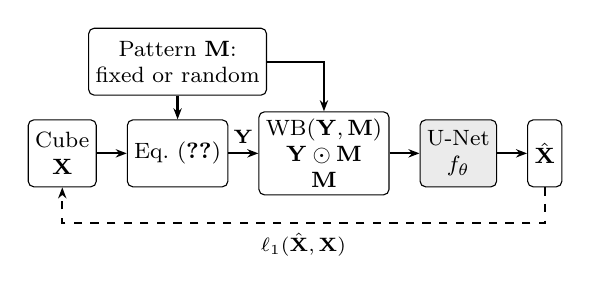
\begin{tikzpicture}[
    box/.style={draw, rounded corners=2pt, align=center, minimum height=0.85cm,
                font=\footnotesize, inner sep=2.5pt},
    arr/.style={-{Stealth[length=4pt]}, thick}]
  \node[box] (cube) {Cube\\$\X$};
  \node[box, right=0.38cm of cube] (sim) {Eq.~\eqref{eq:model}};
  \node[box, above=0.3cm of sim] (rand) {Pattern $\M$:\\fixed or random};
  \node[box, right=0.38cm of sim] (in) {$\wb(\Y,\M)$\\$\Y\odot\M$\\$\M$};
  \node[box, right=0.38cm of in, fill=black!8] (net) {U-Net\\$f_\theta$};
  \node[box, right=0.38cm of net] (out) {$\hat\X$};
  \draw[arr] (cube) -- (sim);
  \draw[arr] (rand) -- (sim);
  \draw[arr] (rand) -| (in);
  \draw[arr] (sim) -- node[above, font=\scriptsize] {$\Y$} (in);
  \draw[arr] (in) -- (net);
  \draw[arr] (net) -- (out);
  \draw[arr, dashed] (out.south) -- ++(0,-0.45) -| node[pos=0.25, below,
       font=\scriptsize] {$\ell_1(\hat\X,\X)$} (cube.south);
\end{tikzpicture}
\caption{Training scheme. For each batch, the mosaic $\Y$ is simulated with
Eq.~\eqref{eq:model} from a pattern $\M$, which is always the same for a
pattern-specific network and a new random balanced pattern for the agnostic
network. The network receives the WB estimate, the sparse cube and the mask
(Eq.~\eqref{eq:input}).}
\label{fig:method}
\end{figure}

% ==========================================================================
\section{Experimental setup}
\label{sec:setup}
% ==========================================================================

\textbf{Data.} CAVE~\cite{yasuma2010} has 32 indoor scenes of
$512\times512$ pixels with 31 bands from 400 to 700\,nm in 10\,nm steps,
stored as 16-bit images that we scale to $[0,1]$. ARAD-1K~\cite{arad2022}
has 950 public training scenes of $482\times512$ pixels with the same 31
bands, indoor and outdoor, captured with a different camera; we obtained it
from a public mirror~\cite{he2023zenodo}. As in~\cite{diaz2023}, we keep 16
bands (400, 420, \dots, 700\,nm). We use two protocols. In the main one,
\emph{CAVE split}, we split CAVE with a fixed random permutation (seed 0)
into 21 training, 3 validation and 8 test scenes: \textit{sponges},
\textit{paints}, \textit{fake and real food}, \textit{stuffed toys},
\textit{pompoms}, \textit{beads}, \textit{fake and real tomatoes} and
\textit{watercolors}. In the \emph{cross-dataset} protocol
(Section~\ref{sec:cross}) we train on 220 ARAD-1K scenes, validate on 30
others and test on all 32 CAVE scenes. We use 250 of the 950 scenes so that
the training set fits in the memory of our laptop. No test scene is used for
training or model selection.

\textbf{Simulation.} Mosaics are simulated with Eq.~\eqref{eq:model}, ideal
filters and no noise ($\N=0$). Every pattern is anchored at the top-left
pixel of the image or patch. The four test patterns are shown in
Fig.~\ref{fig:patterns}.

\textbf{Methods.} We compare five methods: (1) \textbf{WB},
Eq.~\eqref{eq:wb}, with no learning; (2) \textbf{U-Net fixed-IMEC} and
(3) \textbf{U-Net fixed-OSP}, the network of Section~\ref{sec:method}
trained only on IMEC or only on OSP; (4) \textbf{U-Net agnostic}, the same
network trained on random patterns; and (5) \textbf{U-Net no mask (IMEC)}, a
conventional network that receives only $\Y$ (1\,048\,336 parameters) and is
trained on IMEC. Methods (2)--(4) have the same input and architecture, so
any difference between them comes only from the training patterns. Method (5)
represents the usual practice in learned demosaicking.

\textbf{Training.} All networks are trained for 20\,000 iterations with
batches of 32 random $64\times64$ patches, augmented with random flips and
$90^\circ$ rotations. We use Adam~\cite{kingma2015} with a learning rate of
$10^{-3}$ and cosine decay~\cite{loshchilov2017} to $10^{-5}$, and the same
seed for all networks. Every 1\,000 iterations we compute the PSNR on 256
fixed validation patches. For the agnostic network, these patches are split
among 8 fixed random training-type patterns. We keep the checkpoint with the
best validation PSNR. Training took 45 to 55 minutes per network on a laptop
(Apple M5, 16\,GB, PyTorch~\cite{paszke2019} with the MPS backend). Both
protocols use exactly the same settings.

\textbf{Metrics.} Each test scene is reconstructed at full resolution
($512\times512$), clipped to $[0,1]$ and compared with the ground truth. PSNR
is computed over the whole cube with peak value 1. SSIM~\cite{wang2004} is
computed per band with the default $7\times7$ window of
scikit-image~\cite{vanderwalt2014} and then averaged over bands. The spectral
angle mapper (SAM)~\cite{kruse1993} is the angle, in degrees, between the
true and estimated spectrum at each pixel, averaged over pixels. We report
the mean and the sample standard deviation over the test scenes. We also
compute the PSNR of each band, spectral signatures of single pixels, and
error maps on a zoomed crop.

\textbf{Statistics.} The scenes vary much more (about $\pm3.5$\,dB) than the
methods, so for the hypotheses we use paired differences per scene. We
report the mean difference, a 95\% confidence interval (Student $t$ with 7
or 31 degrees of freedom for 8 or 32 scenes) and the number of scenes in
which the comparison holds. With only 8 scenes the intervals of the main
protocol are wide, and we interpret them with caution.

\textbf{Verification of the pipeline.} Our IMEC, BTES and OSP patterns and
our band selection are identical to those of the public MATLAB code
of~\cite{diaz2023}. With their protocol (32 CAVE scenes at $256\times256$,
8-bit data, per-band PSNR), our WB gives 30.45, 30.40 and 30.59\,dB on IMEC,
BTES and OSP, against their 30.57, 30.53 and 30.72\,dB (Table~I
of~\cite{diaz2023}), a constant difference of about 0.13\,dB. The rest of
the report uses our own protocol (full resolution, floating point, PSNR over
the whole cube), so its numbers are not directly comparable with theirs.

% ==========================================================================
\section{Results}
\label{sec:results}
% ==========================================================================

\begin{table*}[t]
\centering
\caption{Results on the 8 CAVE test scenes. PSNR in dB (mean $\pm$ standard
deviation over scenes), SSIM and SAM in degrees (means). Underlined: the
pattern each specific network was trained on. All other cells are unseen
patterns, including every cell of the agnostic network. Bold: best value per
column.}
\label{tab:main}
\footnotesize
\setlength{\tabcolsep}{2.2pt}
\begin{tabular}{|l|ccc|ccc|ccc|ccc|}
\hline
& \multicolumn{3}{c|}{IMEC} & \multicolumn{3}{c|}{OSP}
& \multicolumn{3}{c|}{BTES} & \multicolumn{3}{c|}{Random} \\
Method & PSNR$\uparrow$ & SSIM$\uparrow$ & SAM$\downarrow$
       & PSNR$\uparrow$ & SSIM$\uparrow$ & SAM$\downarrow$
       & PSNR$\uparrow$ & SSIM$\uparrow$ & SAM$\downarrow$
       & PSNR$\uparrow$ & SSIM$\uparrow$ & SAM$\downarrow$ \\
\hline
WB~\cite{brauers2006}
  & 31.99$\pm$3.79 & 0.927 & 4.96
  & 32.13$\pm$3.79 & 0.928 & 4.93
  & 31.98$\pm$3.78 & 0.927 & 4.97
  & 31.99$\pm$3.78 & 0.927 & 4.96 \\
U-Net no mask (IMEC)
  & \seen{35.70$\pm$3.81} & \seen{0.961} & \seen{4.59}
  & 20.75$\pm$3.59 & 0.692 & 26.44
  & 19.76$\pm$3.59 & 0.672 & 35.36
  & 20.24$\pm$3.50 & 0.698 & 28.59 \\
U-Net fixed-IMEC
  & \seen{\textbf{36.64}$\pm$3.49} & \seen{\textbf{0.967}} & \seen{4.18}
  & 29.25$\pm$2.40 & 0.702 & 14.44
  & 28.77$\pm$3.19 & 0.738 & 13.39
  & 29.74$\pm$2.44 & 0.737 & 13.65 \\
U-Net fixed-OSP
  & 25.55$\pm$2.91 & 0.649 & 13.17
  & \seen{\textbf{37.73}$\pm$3.47} & \seen{\textbf{0.975}} & \seen{\textbf{4.14}}
  & 28.90$\pm$2.38 & 0.687 & 13.63
  & 28.95$\pm$2.72 & 0.698 & 13.26 \\
U-Net agnostic (ours)
  & 35.43$\pm$3.33 & 0.964 & 4.94
  & 36.33$\pm$3.44 & 0.970 & 4.69
  & \textbf{36.14}$\pm$3.36 & \textbf{0.970} & \textbf{4.68}
  & \textbf{36.07}$\pm$3.42 & \textbf{0.969} & \textbf{4.77} \\
\hline
\end{tabular}
\end{table*}

Table~\ref{tab:main} gives the results of the CAVE split and
Fig.~\ref{fig:bars} shows the PSNR; Section~\ref{sec:cross} repeats the
experiment across datasets. WB gives practically the same quality on every pattern (31.98 to
32.13\,dB), which shows that the four test patterns are of comparable
difficulty for a pattern-independent method. The learned methods behave
very differently depending on whether the test pattern was seen.
Table~\ref{tab:hyp} summarizes the three hypotheses.

\begin{figure}[t]
\centering
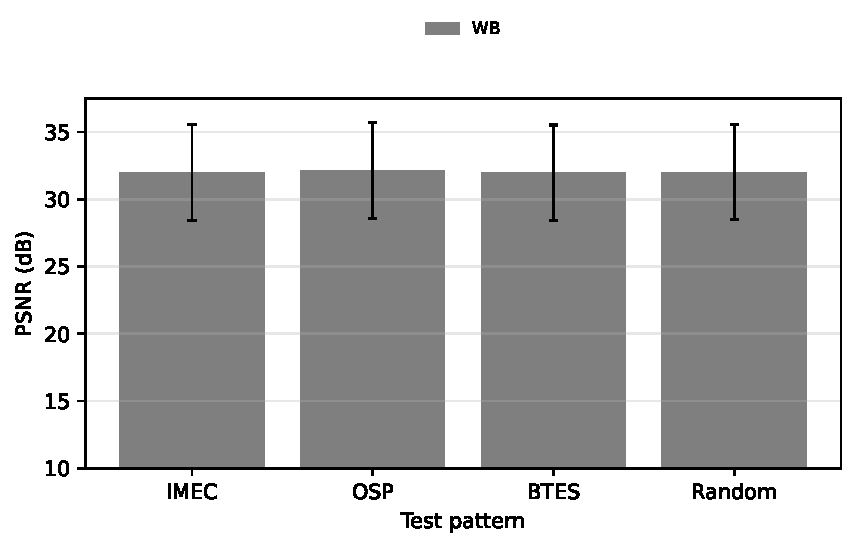
\includegraphics[width=\linewidth]{psnr_bars.pdf}
\caption{Mean PSNR over the 8 test scenes for each method and test pattern
(error bars: standard deviation over scenes). Specific networks are only
good on the pattern they were trained on; the agnostic network (dark red)
is good on all four.}
\label{fig:bars}
\end{figure}

\begin{table}[t]
\centering
\caption{Hypothesis tests (PSNR, dB). H1: drop from the network's own
pattern to the mean of the three unseen patterns. H2 and H3: paired
differences per scene, as mean and 95\% confidence interval. ``Scenes'':
for H2, number of scenes (out of 8) with a gap below 2\,dB / below 1\,dB;
for H3, number of scenes in which the agnostic network is better.}
\label{tab:hyp}
\footnotesize
\setlength{\tabcolsep}{4pt}
\begin{tabular}{|l|l|c|c|}
\hline
Other network & Test MSFA & Mean [95\% CI] & Scenes \\
\hline
\multicolumn{4}{|l|}{\textbf{H1}: own pattern $-$ unseen patterns} \\
\hline
Fixed-IMEC     & 3 unseen & 7.38  & -- \\
Fixed-OSP      & 3 unseen & 9.94  & -- \\
No mask (IMEC) & 3 unseen & 15.45 & -- \\
\hline
\multicolumn{4}{|l|}{\textbf{H2}: specific $-$ agnostic, on the specific pattern} \\
\hline
Fixed-IMEC & IMEC & 1.21 [0.66, 1.75] & 8 / 2 \\
Fixed-OSP  & OSP  & 1.40 [0.88, 1.93] & 5 / 3 \\
\hline
\multicolumn{4}{|l|}{\textbf{H3}: agnostic $-$ other method, on unseen patterns} \\
\hline
Fixed-IMEC & OSP    & 7.08 [5.39, 8.77]  & 8 \\
Fixed-IMEC & BTES   & 7.37 [5.54, 9.20]  & 8 \\
Fixed-IMEC & Random & 6.33 [4.86, 7.80]  & 8 \\
Fixed-OSP  & IMEC   & 9.89 [6.79, 12.98] & 8 \\
Fixed-OSP  & BTES   & 7.25 [5.36, 9.13]  & 8 \\
Fixed-OSP  & Random & 7.12 [5.27, 8.97]  & 8 \\
WB         & IMEC   & 3.44 [1.71, 5.16]  & 7 \\
WB         & OSP    & 4.20 [2.22, 6.18]  & 8 \\
WB         & BTES   & 4.16 [2.29, 6.03]  & 8 \\
WB         & Random & 4.08 [2.20, 5.95]  & 8 \\
\hline
\end{tabular}
\end{table}

\subsection{H1: specific networks fail on unseen patterns}

H1 holds clearly. Fixed-IMEC reaches 36.64\,dB on IMEC but only 28.77 to
29.74\,dB on the other patterns, a mean drop of 7.38\,dB. Fixed-OSP drops by
9.94\,dB, from 37.73 to 25.55--28.95\,dB. The conventional network without
mask drops by 15.45\,dB, to about 20\,dB. All three end up \emph{below} WB,
a method with no learning at all, by 2.2 to 12.2\,dB. The spectral error
grows even more. SAM goes from about $4^\circ$ to $13$--$14^\circ$ for the
fixed networks and to $26$--$35^\circ$ for the network without mask, so the
reconstructed spectra are no longer useful. Two observations explain this.
First, the conventional network has no access to the pattern, so on a new
MSFA it assigns each measurement to the wrong band. Second, the fixed
networks do receive the mask but still fail. A network that always sees the
same pattern learns to ignore the mask and memorizes the pattern. Giving the
mask is therefore not enough: the network must also be trained on many
patterns.

\subsection{H2: the price of generality}

On its own pattern, each specific network is better than the agnostic one.
The gap is 1.21\,dB on IMEC (36.64 vs.\ 35.43\,dB) and 1.40\,dB on OSP
(37.73 vs.\ 36.33\,dB). Both 95\% intervals, [0.66, 1.75] and [0.88, 1.93],
lie below 2\,dB, so H2 holds with the 2\,dB threshold of our project plan.
It does not hold with the stricter 1\,dB threshold of our written proposal,
because both intervals lie mostly above 1\,dB. Per scene, the gap is below
2\,dB in all 8 scenes on IMEC and in 5 of 8 on OSP, and below 1\,dB in only
2 and 3 scenes. In one scene (IMEC) the agnostic network is even better than
the specific one, by 0.19\,dB. SSIM tells the same story (0.964 vs.\ 0.967
and 0.970 vs.\ 0.975). The spectral gap is somewhat larger: SAM rises from
$4.18^\circ$ to $4.94^\circ$ on IMEC and from $4.14^\circ$ to $4.69^\circ$ on
OSP.

The agnostic network is also compared with the conventional network without
mask, which is what a practitioner would train today for an IMEC camera. On
IMEC the two are almost equal (35.43 vs.\ 35.70\,dB, a mean difference of
0.27\,dB that changes sign across scenes, from $-2.85$ to $+1.53$\,dB). In
other words, a single agnostic network matches the conventional IMEC network
on IMEC and also works on every other pattern.

\subsection{H3: generalization to unseen patterns}

H3 holds in every case. On patterns not seen by the specific networks, the
agnostic network is better by 6.33 to 9.89\,dB on average, and it is better
in all 8 scenes in each of the six comparisons. It also improves on WB by
3.44 to 4.20\,dB on average. This advantage holds in 31 of the 32
scene--pattern pairs; the exception is \textit{stuffed toys} on IMEC (35.22
vs.\ 35.37\,dB), a smooth scene where WB is already strong. The agnostic
network's quality is almost constant across patterns (35.43 to 36.33\,dB).
Like the specific networks and like~\cite{diaz2023}, it performs better with
OSP than with IMEC, which agrees with the more uniform spatio-spectral sampling
of OSP. Fixed-OSP is also better on its pattern than fixed-IMEC on its own
(37.73 vs.\ 36.64\,dB).

\subsection{Cross-dataset validation: training on ARAD-1K}
\label{sec:cross}

\begin{table}[t]
\centering
\caption{Cross-dataset protocol: training on ARAD-1K, testing on the 32 CAVE
scenes (mean PSNR in dB). Underlined: own training pattern. Bold: best per
column.}
\label{tab:arad}
\footnotesize
\setlength{\tabcolsep}{3.5pt}
\begin{tabular}{|l|c|c|c|c|}
\hline
Method & IMEC & OSP & BTES & Random \\
\hline
WB (no learning)      & 33.56 & 33.75 & 33.55 & 33.55 \\
U-Net no mask (IMEC)  & \seen{33.86} & 23.56 & 22.33 & 22.82 \\
U-Net fixed-IMEC      & \seen{\textbf{36.30}} & 30.84 & 31.02 & 31.26 \\
U-Net fixed-OSP       & 29.63 & \seen{\textbf{36.48}} & 30.77 & 30.76 \\
U-Net agnostic (ours) & 34.97 & 35.47 & \textbf{35.29} & \textbf{35.31} \\
\hline
\end{tabular}
\end{table}

The CAVE split has only 8 test scenes and uses one dataset for training and
testing. We therefore retrained the four networks on ARAD-1K, with the same
settings, and tested them on all 32 CAVE scenes (Table~\ref{tab:arad}). The
three hypotheses hold again. \textbf{H1}: fixed-IMEC, fixed-OSP and the
network without mask lose 5.26, 6.09 and 10.96\,dB on unseen patterns and
fall below WB. \textbf{H2}: the gap to the specialist is 1.33\,dB on IMEC
(95\% CI [1.16, 1.50]) and 1.01\,dB on OSP ([0.75, 1.27]). It is below
2\,dB in 31 of 32 scenes on both patterns and below 1\,dB in 7 and 14
scenes, so H2 again holds with 2\,dB but not with 1\,dB. \textbf{H3}: on
unseen patterns the agnostic network beats the specialists by 4.05 to
5.34\,dB, in all 32 scenes of the six comparisons, and WB by 1.41 to
1.76\,dB (intervals from [0.37, 2.44] to [0.69, 2.84]). On IMEC it is now
also better than the network without mask, by 1.10\,dB ([0.66, 1.55], 25 of
32 scenes).

The margin over WB is smaller than in the CAVE split. In six scenes
(\textit{cd}, \textit{clay}, \textit{superballs}, \textit{pompoms},
\textit{balloons}, \textit{stuffed toys}) the agnostic network is below WB on
all four patterns, by up to 7.2\,dB, and its mean SAM, like that of the
specialists on their own pattern (11.2 to $13.4^\circ$), is about twice that
of WB ($5.5^\circ$). This is a dataset gap that affects every learned
method, not the agnostic network alone: in these six scenes the specialists
are also below WB on their own pattern, and on the 8 test scenes of the CAVE
split the networks trained on ARAD-1K lose 2.5 to 4.0\,dB compared with the
same networks trained on CAVE, while WB is unchanged. Most of the additional
error lies in bright pixels, so the dark backgrounds of CAVE are not the
cause. Normalized by their
mean, CAVE spectra change about twice as much between adjacent bands as
ARAD-1K spectra (mean absolute difference 0.195 vs.\ 0.100), so the networks
probably learn a spectral prior that is too smooth for CAVE. Since all
networks share the same training data, the comparison between them, and
therefore H1--H3, remains valid.

\subsection{Per-band accuracy and spectral fidelity}

\begin{figure*}[t]
\centering
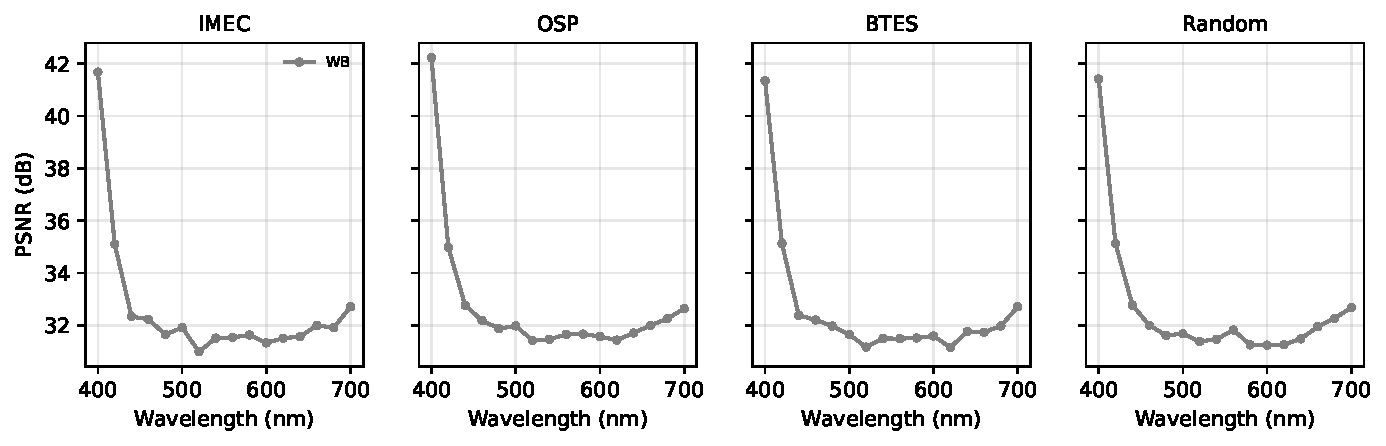
\includegraphics[width=\linewidth]{psnr_per_band.pdf}
\caption{PSNR of each band, averaged over the 8 test scenes, for each test
pattern. The agnostic network (dark red) gives a flat curve around 35--37\,dB
on all patterns. The specific networks are only above WB on their own
pattern.}
\label{fig:bands}
\end{figure*}

Fig.~\ref{fig:bands} shows the PSNR per band. All methods reach their highest
PSNR at 400\,nm, a dark band in CAVE with small absolute errors. On the other
bands, the agnostic network stays between about 35 and 37\,dB for every
pattern, 3 to 5\,dB above WB. Each specific network is the best or close to
the best in every band of its own pattern, and below WB in every band of the
other patterns. The degradation is not uniform: fixed-OSP on IMEC loses
accuracy steadily with wavelength, from 36.5\,dB at 400\,nm to about 23\,dB
at 640\,nm, consistent with bands being confused with each other.
Fig.~\ref{fig:spectra} shows reconstructed spectra of two pixels under OSP.
WB oscillates around the true spectrum, a spectral form of the zipper
artifact, because neighboring bands are interpolated from samples at
different positions. The network without mask loses the shape of the
spectrum, while the networks with mask follow the reference.

\begin{figure}[t]
\centering
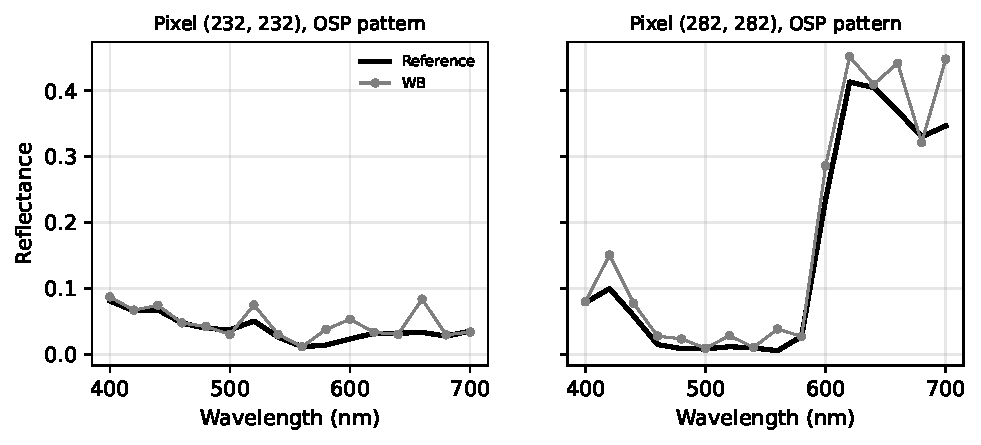
\includegraphics[width=\linewidth]{spectra.pdf}
\caption{Reconstructed spectra of two pixels of the \textit{beads} scene
with the OSP pattern. WB oscillates around the reference and the
network without mask (trained on IMEC) loses the spectral shape; the
agnostic network follows the reference.}
\label{fig:spectra}
\end{figure}

\subsection{Visual inspection}

\begin{figure*}[t]
\centering
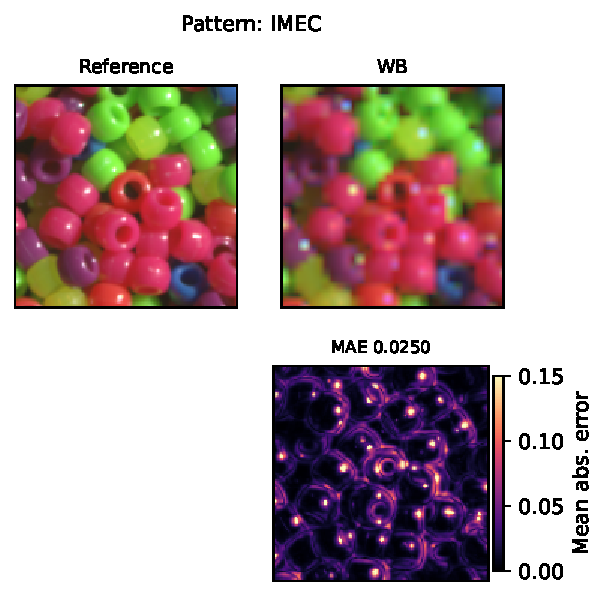
\includegraphics[width=0.49\linewidth]{visual_imec.pdf}\hfill
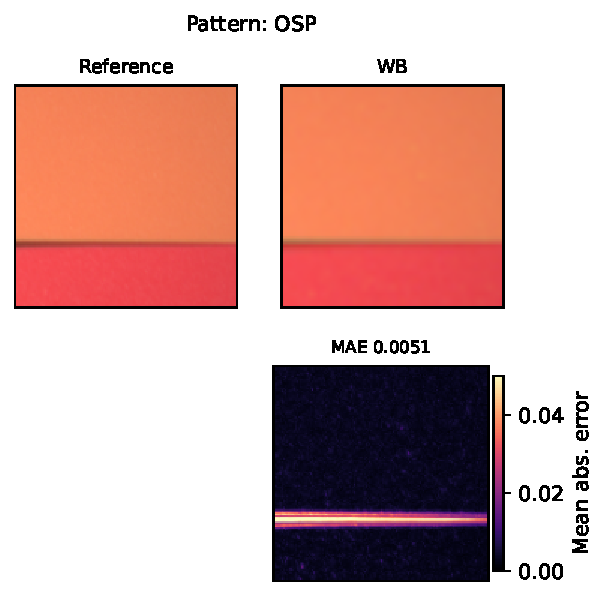
\includegraphics[width=0.49\linewidth]{visual_osp.pdf}
\caption{Central $128\times128$ crop of the \textit{beads} test scene with
the IMEC (left) and OSP (right) patterns, in false color (bands at 660, 540
and 460\,nm). Top: reconstructions. Bottom: mean absolute error over bands
(MAE of the crop above each map). Networks on an unseen pattern produce
periodic artifacts (fixed-OSP on IMEC, fixed-IMEC on OSP) and false colors
(no mask on OSP); the agnostic network does not.}
\label{fig:visual}
\end{figure*}

Fig.~\ref{fig:visual} shows a crop of \textit{beads}, the hardest test scene
(all methods stay below 32\,dB on it). WB blurs edges, and its error
concentrates on the contours and specular highlights. On an unseen pattern
the specific networks produce structured artifacts: fixed-OSP on IMEC covers
the image with a grid of the period of the filter kernel (zipper), with
twice the crop error of WB (0.052 vs.\ 0.025), and fixed-IMEC on OSP shows a
weaker periodic texture. The network without mask on OSP gives strong false
colors: the beads turn grayish and the error is more than four times that of
WB (0.110). The agnostic network shows neither zipper nor false colors, and
its error (0.024 on IMEC, 0.023 on OSP) is close to that of the specific
network on its own pattern (0.022 and 0.021).

\subsection{Ablation: what the network needs to see}
\label{sec:ablation}

Our first agnostic network received $[\Y,\M]$, as proposed in our project
plan. In short training runs it learned much more slowly than the specific
networks, so we compared several inputs before the final training.
Table~\ref{tab:ablation} reports the results. These runs used 2\,000
iterations and the 3 validation scenes (never the test scenes), so they are
only indicative. With $[\Y,\M]$ the agnostic network stays 3.3 to 4.4\,dB
\emph{below} WB. Feeding the sparse cube, $[\Y\odot\M,\M]$, gains only about
1\,dB. A third option kept WB as a fixed base and let the network learn a
residual correction. It collapsed to exactly WB: within about 20 iterations,
all ReLU units of the last hidden layer died and the gradients vanished,
because the target residual is tiny (median $0.0016$) compared with the Adam
step. This happened even when the last layer was initialized to zero. Giving
the WB estimate as an \emph{input}, Eq.~\eqref{eq:input}, solved the
problem: the agnostic network jumped from 28.3 to 34.6\,dB on IMEC, already
2\,dB above WB. Our interpretation is that WB already performs the
pattern-dependent part of the work (which sample belongs to which band, and
how to spread it), so the network only has to learn a pattern-independent
refinement. Since this input was also better for the specific networks
(fixed-IMEC 36.12\,dB at 2\,000 iterations), we used it for all networks so
that they differ only in their training patterns.

\begin{table}[t]
\centering
\caption{Input ablation for the agnostic network (short runs: 2\,000
iterations, 3 validation scenes, PSNR in dB). Indicative only; the final
networks were trained 10 times longer.}
\label{tab:ablation}
\footnotesize
\setlength{\tabcolsep}{3.5pt}
\begin{tabular}{|l|c|c|c|c|}
\hline
Input / method & IMEC & OSP & BTES & Random \\
\hline
WB (no learning)            & 32.60 & 32.66 & 32.60 & 32.60 \\
\hline
$[\Y,\M]$ (proposal)          & 28.26 & 28.45 & 29.11 & 29.34 \\
$[\Y\odot\M,\M]$             & 29.89 & 29.80 & 29.75 & 29.86 \\
WB + learned residual       & 32.60 & 32.66 & 32.60 & 32.60 \\
$[\wb,\Y\odot\M,\M]$ (ours)  & \textbf{34.61} & \textbf{35.07} & \textbf{35.02} & \textbf{34.89} \\
\hline
\end{tabular}
\end{table}

The short runs also explain why the specific networks receive the mask. A
U-Net with two poolings is equivariant to shifts of 4 pixels, but OSP
repeats every 16 rows, so without the mask the network cannot know the row
phase of the pattern. A mask-less fixed-OSP network performed the same with
the pattern shifted by 4 rows (33.40 vs.\ 33.42\,dB), and the mask improved
it by 1.45\,dB. A mask-less specialist would thus be artificially weak on OSP
and would hide part of the H2 gap.

\subsection{Training behavior}

In the CAVE split, the validation PSNR (curves in the repository) of
fixed-IMEC plateaus at about 35.5\,dB after 8\,000 iterations, that of the
agnostic network at 34.8\,dB after 13\,000 and that of fixed-OSP at 37.3\,dB
after 15\,000, while the training loss keeps decreasing. Between the short
runs and the final training (10 times more iterations), the H2 gap on IMEC
changed only from about 1.5 to 1.21\,dB, and with ten times more training
scenes (ARAD-1K) the gaps are similar (1.33 and 1.01\,dB). More iterations
or more data alone are therefore unlikely to close the gap; the capacity of
the network may be the limit.

% ==========================================================================
\section{Discussion}
\label{sec:discussion}
% ==========================================================================

\textbf{What the results mean.} Training one network per pattern has a
hidden cost: on a new MSFA the network is \emph{worse than bilinear
interpolation} and produces zipper and false-color artifacts. A single
network conditioned on the mask and trained on random balanced patterns
avoids this on four very different MSFAs, including a non-periodic lattice
(OSP), at a cost of 1.0 to 1.4\,dB against a specialist on the specialist's
pattern. This has three uses: (i) candidate MSFAs can be compared with one
trained network instead of one per pattern, which addresses the limitation
stated in~\cite{diaz2023}; (ii) one model can serve sensors with different
layouts, or a sensor whose layout differs slightly from its nominal design;
(iii) when a camera is fixed, the agnostic network is a natural starting
point for fine-tuning on its pattern (not tested here).

\textbf{Why it works.} Two ingredients are both necessary. The mask, or a
pattern-aware interpolation, must reach the network; otherwise the network
cannot tell bands apart on a new pattern. The training patterns must also
vary; otherwise the network learns to ignore the mask. Our fixed networks
have the mask and still fail on new patterns, and our agnostic network with
input $[\Y,\M]$ has varied patterns but learns slowly. Giving WB as input
combines the two in the simplest way: a classical, pattern-independent
operator (normalized convolution) handles the geometry of the pattern, and
the network learns the image prior.

\textbf{Originality.} Random-pattern training has been shown for RGB
CFAs~\cite{bourrier2022}, mask conditioning with random masks is standard in
inpainting~\cite{liu2018}, and normalized convolution~\cite{knutsson1993}
predates deep learning. Our contribution is to bring these ideas to 16-band
MSFA demosaicking, where networks are still trained per
pattern~\cite{feng2021,diaz2023}, and to identify what makes them work in
this harder setting. In our ablation, a sparse-cube input, similar to the
one used for RGB in~\cite{bourrier2022}, learns too slowly with 16 bands,
and a pattern-aware interpolation as input solves this. We also give a
controlled measurement of the cost of pattern dependence, with specialists
and an agnostic network that differ only in their training patterns.

\textbf{Limitations.} Our conclusions are limited by the following choices.
(1) \emph{Data}: the main protocol tests on only 8 CAVE scenes. The
cross-dataset protocol confirms H1--H3 on 32 scenes, but shows that every
learned method loses accuracy, especially spectral accuracy, when the test
data differ from the training data; with ARAD-1K training, the margin over
WB shrinks to 1.4--1.8\,dB and disappears in 6 of 32 scenes. (2)
\emph{Simulation}: we assume ideal narrow-band filters and no noise. Real
IMEC filters overlap spectrally and real sensors add noise, which would make
the problem harder for all methods. (3) \emph{Patterns}: all test and
training patterns have 16 bands and one band per $4\times4$ block. We have
not tested patterns with repeated bands or other kernel sizes, which the
agnostic network may not handle. (4) \emph{Baselines}: we compare networks
with the same architecture, which isolates the effect of the training
patterns, but we do not compare with state-of-the-art demosaicking networks
such as TRevSCI or MCAN, nor with stronger classical methods such as PPID.
For reference, TRevSCI reports 35.8, 37.6 and 38.8\,dB on IMEC, BTES and
OSP~\cite{diaz2023}, but with a different protocol, so these numbers are not
directly comparable with ours. (5) \emph{Statistics}: each network was
trained once, with one seed, so we do not measure the variation between
training runs.

\textbf{Future work.} Natural next steps are: training on several datasets
to reduce the dataset gap, adding noise and real filter responses, testing patterns with other
sizes and with repeated bands, fine-tuning the agnostic network on a fixed
pattern, increasing the network capacity to reduce the H2 gap, and using the
agnostic network as a fast evaluator inside an MSFA design loop.

% ==========================================================================
\section{Conclusion}
\label{sec:conclusion}
% ==========================================================================

We studied whether one learned demosaicking network can serve any
multispectral filter array. Networks trained for a single pattern, with or
without the mask as input, lose 7.4 to 15.5\,dB on unseen patterns and fall
below bilinear interpolation (H1). A U-Net that receives a bilinear
estimate, the sparse measurements and the mask, and is trained on random
balanced patterns, stays within 1.2 to 1.4\,dB of a specialist on the
specialist's own pattern (H2 with a 2\,dB threshold, though not with 1\,dB)
and outperforms the specialists by 6.3 to 9.9\,dB and bilinear interpolation
by 3.4 to 4.2\,dB on unseen patterns (H3). Training on ARAD-1K and testing
on all 32 CAVE scenes confirms the three hypotheses, although the change of
dataset hurts every learned method and reduces the margin over bilinear
interpolation to 1.4--1.8\,dB. The key design choice is to give the network
a pattern-aware interpolation as input. A single network can therefore
replace one network per pattern at a modest cost in accuracy, which makes
learned demosaicking practical for MSFA design and for cameras with
different filter layouts.

% ==========================================================================
\section{Data, code and acknowledgments}
\label{sec:ack}
% ==========================================================================

All code (simulator, baselines, networks, training, evaluation and
figures) and all results reported here are available at\\
{\footnotesize\url{https://github.com/GonzaMichea/Multiespectral-Demosaicking}}.\\
The tables
and figures are generated from the files in \texttt{results/} and
\texttt{results\_arad/}, and both protocols can be reproduced with
\texttt{scripts/run\_all.sh}. We thank the authors of the CAVE~\cite{yasuma2010}
and ARAD-1K~\cite{arad2022} datasets and Diaz et
al.~\cite{diaz2023} for their public MATLAB code, which we used to verify our
patterns and our WB baseline. The software is based on
PyTorch~\cite{paszke2019}, NumPy~\cite{harris2020},
SciPy~\cite{virtanen2020}, scikit-image~\cite{vanderwalt2014} and
Matplotlib~\cite{hunter2007}.

% References.
% -----------
% Smaller font for the references, as in IEEE journals.
\begingroup
\small
\bibliographystyle{IEEEbib}
\bibliography{strings,refs}
\endgroup

\end{document}
